% Created by tikzDevice version 0.12.3.1 on 2022-09-02 10:38:07
% !TEX encoding = UTF-8 Unicode
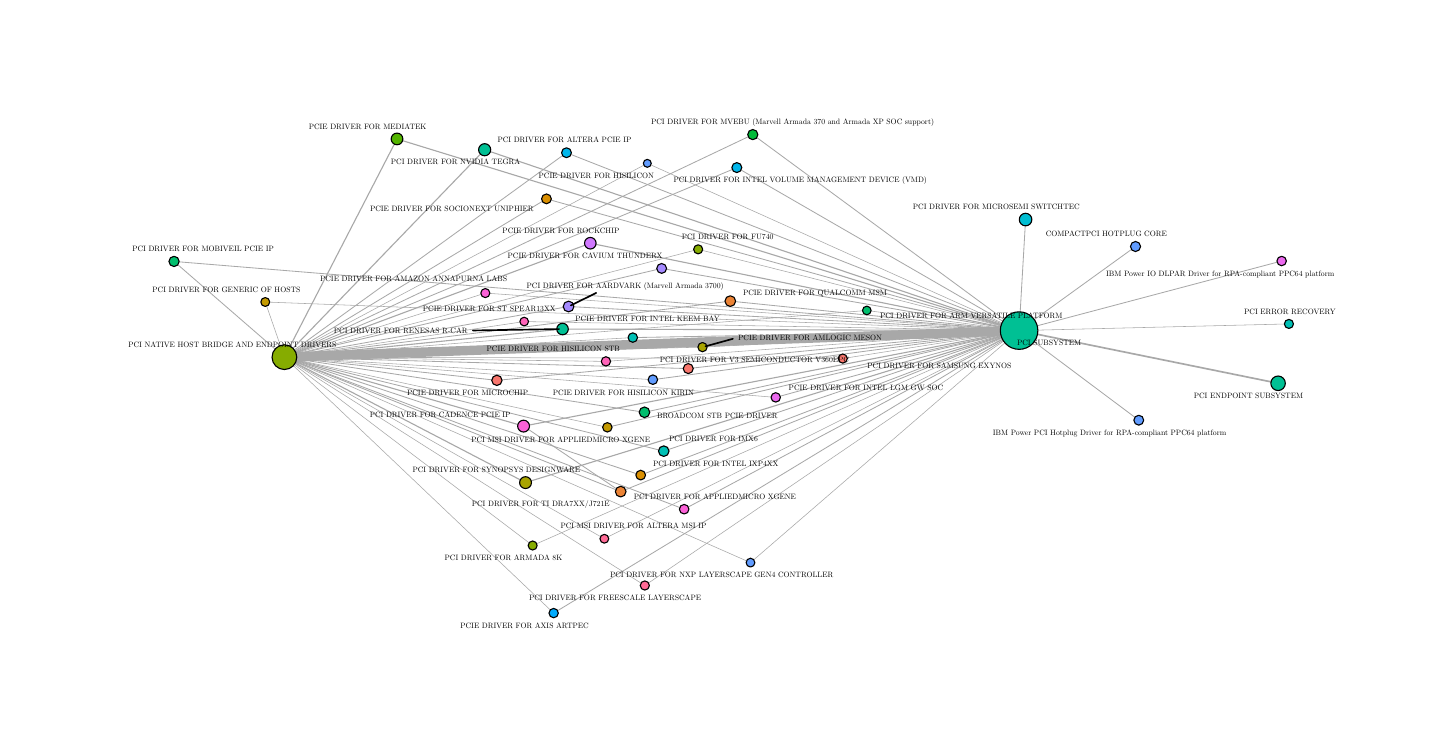
\begin{tikzpicture}[x=1pt,y=1pt]
\definecolor{fillColor}{RGB}{255,255,255}
\path[use as bounding box,fill=fillColor,fill opacity=0.00] (0,0) rectangle (505.89,252.94);
\begin{scope}
\path[clip] (  0.00,  0.00) rectangle (505.89,252.94);
\definecolor{fillColor}{RGB}{255,255,255}

\path[fill=fillColor] (  0.00,  0.00) rectangle (505.89,252.94);
\end{scope}
\begin{scope}
\path[clip] ( 32.75, 32.75) rectangle (475.89,222.94);
\definecolor{drawColor}{gray}{0.66}

\path[draw=drawColor,line width= 0.3pt,line join=round] (222.88,113.96) -- ( 92.77,133.88);

\path[draw=drawColor,line width= 0.3pt,line join=round] (222.88,113.96) -- (358.25,143.48);

\path[draw=drawColor,line width= 0.3pt,line join=round] (400.32,173.86) -- (358.25,143.48);

\path[draw=drawColor,line width= 0.3pt,line join=round] (453.12,168.62) -- (358.25,143.48);

\path[draw=drawColor,line width= 0.3pt,line join=round] (401.49,111.10) -- (358.25,143.48);

\path[draw=drawColor,line width= 0.3pt,line join=round] (195.45,152.18) -- ( 92.77,133.88);

\path[draw=drawColor,line width= 0.3pt,line join=round] (195.45,152.18) -- (358.25,143.48);

\path[draw=drawColor,line width= 0.3pt,line join=round] (194.70,207.75) -- ( 92.77,133.88);

\path[draw=drawColor,line width= 0.3pt,line join=round] (194.70,207.75) -- (358.25,143.48);

\path[draw=drawColor,line width= 0.3pt,line join=round] (237.22, 78.94) -- ( 92.77,133.88);

\path[draw=drawColor,line width= 0.3pt,line join=round] (237.22, 78.94) -- (358.25,143.48);

\path[draw=drawColor,line width= 0.2pt,line join=round] (303.22,150.75) -- ( 92.77,133.88);

\path[draw=drawColor,line width= 0.2pt,line join=round] (303.22,150.75) -- (358.25,143.48);

\path[draw=drawColor,line width= 0.2pt,line join=round] (182.47, 65.82) -- ( 92.77,133.88);

\path[draw=drawColor,line width= 0.2pt,line join=round] (182.47, 65.82) -- (358.25,143.48);

\path[draw=drawColor,line width= 0.3pt,line join=round] (179.19,108.96) -- (214.28, 85.29);

\path[draw=drawColor,line width= 0.4pt,line join=round] (179.19,108.96) -- ( 92.77,133.88);

\path[draw=drawColor,line width= 0.4pt,line join=round] (179.19,108.96) -- (358.25,143.48);

\path[draw=drawColor,line width= 0.2pt,line join=round] (223.00, 51.37) -- ( 92.77,133.88);

\path[draw=drawColor,line width= 0.2pt,line join=round] (223.00, 51.37) -- (358.25,143.48);

\path[draw=drawColor,line width= 0.2pt,line join=round] (242.28,172.84) -- ( 92.77,133.88);

\path[draw=drawColor,line width= 0.2pt,line join=round] (242.28,172.84) -- (358.25,143.48);

\path[draw=drawColor,line width= 0.2pt,line join=round] ( 85.85,153.81) -- ( 92.77,133.88);

\path[draw=drawColor,line width= 0.2pt,line join=round] ( 85.85,153.81) -- (358.25,143.48);

\path[draw=drawColor,line width= 0.3pt,line join=round] (229.84, 99.92) -- ( 92.77,133.88);

\path[draw=drawColor,line width= 0.3pt,line join=round] (229.84, 99.92) -- (358.25,143.48);

\path[draw=drawColor,line width= 0.3pt,line join=round] (221.51, 91.26) -- ( 92.77,133.88);

\path[draw=drawColor,line width= 0.3pt,line join=round] (221.51, 91.26) -- (358.25,143.48);

\path[draw=drawColor,line width= 0.3pt,line join=round] (256.25,202.38) -- ( 92.77,133.88);

\path[draw=drawColor,line width= 0.3pt,line join=round] (256.25,202.38) -- (358.25,143.48);

\path[draw=drawColor,line width= 0.3pt,line join=round] (360.59,183.60) -- (358.25,143.48);

\path[draw=drawColor,line width= 0.3pt,line join=round] ( 52.89,168.47) -- ( 92.77,133.88);

\path[draw=drawColor,line width= 0.3pt,line join=round] ( 52.89,168.47) -- (358.25,143.48);

\path[draw=drawColor,line width= 0.3pt,line join=round] (262.02,214.30) -- ( 92.77,133.88);

\path[draw=drawColor,line width= 0.3pt,line join=round] (262.02,214.30) -- (358.25,143.48);

\path[draw=drawColor,line width= 0.4pt,line join=round] (165.13,208.83) -- ( 92.77,133.88);

\path[draw=drawColor,line width= 0.4pt,line join=round] (165.13,208.83) -- (358.25,143.48);

\path[draw=drawColor,line width= 0.2pt,line join=round] (261.19, 59.64) -- ( 92.77,133.88);

\path[draw=drawColor,line width= 0.2pt,line join=round] (261.19, 59.64) -- (358.25,143.48);

\path[draw=drawColor,line width= 0.4pt,line join=round] (193.27,144.04) -- ( 92.77,133.88);

\path[draw=drawColor,line width= 0.4pt,line join=round] (193.27,144.04) -- (358.25,143.48);

\path[draw=drawColor,line width= 0.2pt,line join=round] (294.52,133.37) -- ( 92.77,133.88);

\path[draw=drawColor,line width= 0.2pt,line join=round] (294.52,133.37) -- (358.25,143.48);

\path[draw=drawColor,line width= 0.4pt,line join=round] (179.90, 88.55) -- ( 92.77,133.88);

\path[draw=drawColor,line width= 0.4pt,line join=round] (179.90, 88.55) -- (358.25,143.48);

\path[draw=drawColor,line width= 0.3pt,line join=round] (214.28, 85.29) -- ( 92.77,133.88);

\path[draw=drawColor,line width= 0.3pt,line join=round] (214.28, 85.29) -- (358.25,143.48);

\path[draw=drawColor,line width= 0.3pt,line join=round] (238.70,129.75) -- ( 92.77,133.88);

\path[draw=drawColor,line width= 0.3pt,line join=round] (238.70,129.75) -- (358.25,143.48);

\path[draw=drawColor,line width= 0.6pt,line join=round] (451.83,124.44) -- (358.25,143.48);

\path[draw=drawColor,line width= 0.2pt,line join=round] (455.75,145.89) -- (358.25,143.48);

\path[draw=drawColor,line width= 0.2pt,line join=round] (208.38, 68.26) -- ( 92.77,133.88);

\path[draw=drawColor,line width= 0.2pt,line join=round] (208.38, 68.26) -- (358.25,143.48);

\path[draw=drawColor,line width= 0.2pt,line join=round] (209.46,108.53) -- ( 92.77,133.88);

\path[draw=drawColor,line width= 0.3pt,line join=round] (209.46,108.53) -- (358.25,143.48);

\path[draw=drawColor,line width= 3.4pt,line join=round] ( 92.77,133.88) -- (358.25,143.48);

\path[draw=drawColor,line width= 0.2pt,line join=round] ( 92.77,133.88) -- (165.37,157.03);

\path[draw=drawColor,line width= 0.2pt,line join=round] ( 92.77,133.88) -- (243.85,137.50);

\path[draw=drawColor,line width= 0.2pt,line join=round] ( 92.77,133.88) -- (190.06, 41.40);

\path[draw=drawColor,line width= 0.3pt,line join=round] ( 92.77,133.88) -- (229.09,165.94);

\path[draw=drawColor,line width= 0.2pt,line join=round] ( 92.77,133.88) -- (223.90,203.92);

\path[draw=drawColor,line width= 0.2pt,line join=round] ( 92.77,133.88) -- (225.91,125.74);

\path[draw=drawColor,line width= 0.2pt,line join=round] ( 92.77,133.88) -- (208.95,132.35);

\path[draw=drawColor,line width= 0.2pt,line join=round] ( 92.77,133.88) -- (218.66,140.95);

\path[draw=drawColor,line width= 0.2pt,line join=round] ( 92.77,133.88) -- (270.31,119.34);

\path[draw=drawColor,line width= 0.4pt,line join=round] ( 92.77,133.88) -- (133.46,212.73);

\path[draw=drawColor,line width= 0.3pt,line join=round] ( 92.77,133.88) -- (169.55,125.50);

\path[draw=drawColor,line width= 0.3pt,line join=round] ( 92.77,133.88) -- (253.89,154.13);

\path[draw=drawColor,line width= 0.4pt,line join=round] ( 92.77,133.88) -- (203.31,175.05);

\path[draw=drawColor,line width= 0.3pt,line join=round] ( 92.77,133.88) -- (187.46,191.08);

\path[draw=drawColor,line width= 0.2pt,line join=round] ( 92.77,133.88) -- (179.41,146.74);

\path[draw=drawColor,line width= 0.2pt,line join=round] (358.25,143.48) -- (165.37,157.03);

\path[draw=drawColor,line width= 0.2pt,line join=round] (358.25,143.48) -- (243.85,137.50);

\path[draw=drawColor,line width= 0.3pt,line join=round] (358.25,143.48) -- (190.06, 41.40);

\path[draw=drawColor,line width= 0.3pt,line join=round] (358.25,143.48) -- (229.09,165.94);

\path[draw=drawColor,line width= 0.2pt,line join=round] (358.25,143.48) -- (223.90,203.92);

\path[draw=drawColor,line width= 0.3pt,line join=round] (358.25,143.48) -- (225.91,125.74);

\path[draw=drawColor,line width= 0.2pt,line join=round] (358.25,143.48) -- (208.95,132.35);

\path[draw=drawColor,line width= 0.3pt,line join=round] (358.25,143.48) -- (218.66,140.95);

\path[draw=drawColor,line width= 0.3pt,line join=round] (358.25,143.48) -- (270.31,119.34);

\path[draw=drawColor,line width= 0.4pt,line join=round] (358.25,143.48) -- (133.46,212.73);

\path[draw=drawColor,line width= 0.3pt,line join=round] (358.25,143.48) -- (169.55,125.50);

\path[draw=drawColor,line width= 0.3pt,line join=round] (358.25,143.48) -- (253.89,154.13);

\path[draw=drawColor,line width= 0.4pt,line join=round] (358.25,143.48) -- (203.31,175.05);

\path[draw=drawColor,line width= 0.3pt,line join=round] (358.25,143.48) -- (187.46,191.08);

\path[draw=drawColor,line width= 0.2pt,line join=round] (358.25,143.48) -- (179.41,146.74);
\definecolor{drawColor}{RGB}{0,0,0}
\definecolor{fillColor}{RGB}{0,190,109}

\path[draw=drawColor,line width= 0.4pt,line join=round,line cap=round,fill=fillColor] (222.88,113.96) circle (  1.91);
\definecolor{fillColor}{RGB}{97,156,255}

\path[draw=drawColor,line width= 0.4pt,line join=round,line cap=round,fill=fillColor] (400.32,173.86) circle (  1.82);
\definecolor{fillColor}{RGB}{236,105,239}

\path[draw=drawColor,line width= 0.4pt,line join=round,line cap=round,fill=fillColor] (453.12,168.62) circle (  1.71);
\definecolor{fillColor}{RGB}{97,156,255}

\path[draw=drawColor,line width= 0.4pt,line join=round,line cap=round,fill=fillColor] (401.49,111.10) circle (  1.78);
\definecolor{fillColor}{RGB}{165,138,255}

\path[draw=drawColor,line width= 0.4pt,line join=round,line cap=round,fill=fillColor] (195.45,152.18) circle (  1.94);
\definecolor{fillColor}{RGB}{0,182,235}

\path[draw=drawColor,line width= 0.4pt,line join=round,line cap=round,fill=fillColor] (194.70,207.75) circle (  1.78);
\definecolor{fillColor}{RGB}{251,97,215}

\path[draw=drawColor,line width= 0.4pt,line join=round,line cap=round,fill=fillColor] (237.22, 78.94) circle (  1.73);
\definecolor{fillColor}{RGB}{0,190,109}

\path[draw=drawColor,line width= 0.4pt,line join=round,line cap=round,fill=fillColor] (303.22,150.75) circle (  1.56);
\definecolor{fillColor}{RGB}{134,172,0}

\path[draw=drawColor,line width= 0.4pt,line join=round,line cap=round,fill=fillColor] (182.47, 65.82) circle (  1.63);
\definecolor{fillColor}{RGB}{251,97,215}

\path[draw=drawColor,line width= 0.4pt,line join=round,line cap=round,fill=fillColor] (179.19,108.96) circle (  2.14);
\definecolor{fillColor}{RGB}{255,107,150}

\path[draw=drawColor,line width= 0.4pt,line join=round,line cap=round,fill=fillColor] (223.00, 51.37) circle (  1.65);
\definecolor{fillColor}{RGB}{134,172,0}

\path[draw=drawColor,line width= 0.4pt,line join=round,line cap=round,fill=fillColor] (242.28,172.84) circle (  1.64);
\definecolor{fillColor}{RGB}{196,154,0}

\path[draw=drawColor,line width= 0.4pt,line join=round,line cap=round,fill=fillColor] ( 85.85,153.81) circle (  1.61);
\definecolor{fillColor}{RGB}{0,192,181}

\path[draw=drawColor,line width= 0.4pt,line join=round,line cap=round,fill=fillColor] (229.84, 99.92) circle (  1.91);
\definecolor{fillColor}{RGB}{218,143,0}

\path[draw=drawColor,line width= 0.4pt,line join=round,line cap=round,fill=fillColor] (221.51, 91.26) circle (  1.75);
\definecolor{fillColor}{RGB}{0,182,235}

\path[draw=drawColor,line width= 0.4pt,line join=round,line cap=round,fill=fillColor] (256.25,202.38) circle (  1.80);
\definecolor{fillColor}{RGB}{0,189,210}

\path[draw=drawColor,line width= 0.4pt,line join=round,line cap=round,fill=fillColor] (360.59,183.60) circle (  2.27);
\definecolor{fillColor}{RGB}{0,190,109}

\path[draw=drawColor,line width= 0.4pt,line join=round,line cap=round,fill=fillColor] ( 52.89,168.47) circle (  1.85);
\definecolor{fillColor}{RGB}{0,186,56}

\path[draw=drawColor,line width= 0.4pt,line join=round,line cap=round,fill=fillColor] (262.02,214.30) circle (  1.84);
\definecolor{fillColor}{RGB}{0,192,148}

\path[draw=drawColor,line width= 0.4pt,line join=round,line cap=round,fill=fillColor] (165.13,208.83) circle (  2.19);
\definecolor{fillColor}{RGB}{97,156,255}

\path[draw=drawColor,line width= 0.4pt,line join=round,line cap=round,fill=fillColor] (261.19, 59.64) circle (  1.58);
\definecolor{fillColor}{RGB}{0,192,148}

\path[draw=drawColor,line width= 0.4pt,line join=round,line cap=round,fill=fillColor] (193.27,144.04) circle (  2.08);
\definecolor{fillColor}{RGB}{248,118,109}

\path[draw=drawColor,line width= 0.4pt,line join=round,line cap=round,fill=fillColor] (294.52,133.37) circle (  1.65);
\definecolor{fillColor}{RGB}{169,164,0}

\path[draw=drawColor,line width= 0.4pt,line join=round,line cap=round,fill=fillColor] (179.90, 88.55) circle (  2.14);
\definecolor{fillColor}{RGB}{235,131,53}

\path[draw=drawColor,line width= 0.4pt,line join=round,line cap=round,fill=fillColor] (214.28, 85.29) circle (  1.93);
\definecolor{fillColor}{RGB}{248,118,109}

\path[draw=drawColor,line width= 0.4pt,line join=round,line cap=round,fill=fillColor] (238.70,129.75) circle (  1.81);
\definecolor{fillColor}{RGB}{0,192,148}

\path[draw=drawColor,line width= 0.4pt,line join=round,line cap=round,fill=fillColor] (451.83,124.44) circle (  2.62);
\definecolor{fillColor}{RGB}{0,192,181}

\path[draw=drawColor,line width= 0.4pt,line join=round,line cap=round,fill=fillColor] (455.75,145.89) circle (  1.64);
\definecolor{fillColor}{RGB}{255,107,150}

\path[draw=drawColor,line width= 0.4pt,line join=round,line cap=round,fill=fillColor] (208.38, 68.26) circle (  1.59);
\definecolor{fillColor}{RGB}{196,154,0}

\path[draw=drawColor,line width= 0.4pt,line join=round,line cap=round,fill=fillColor] (209.46,108.53) circle (  1.70);
\definecolor{fillColor}{RGB}{134,172,0}

\path[draw=drawColor,line width= 0.4pt,line join=round,line cap=round,fill=fillColor] ( 92.77,133.88) circle (  4.47);
\definecolor{fillColor}{RGB}{0,192,148}

\path[draw=drawColor,line width= 0.4pt,line join=round,line cap=round,fill=fillColor] (358.25,143.48) circle (  6.78);
\definecolor{fillColor}{RGB}{251,97,215}

\path[draw=drawColor,line width= 0.4pt,line join=round,line cap=round,fill=fillColor] (165.37,157.03) circle (  1.64);
\definecolor{fillColor}{RGB}{169,164,0}

\path[draw=drawColor,line width= 0.4pt,line join=round,line cap=round,fill=fillColor] (243.85,137.50) circle (  1.67);
\definecolor{fillColor}{RGB}{0,171,253}

\path[draw=drawColor,line width= 0.4pt,line join=round,line cap=round,fill=fillColor] (190.06, 41.40) circle (  1.69);
\definecolor{fillColor}{RGB}{165,138,255}

\path[draw=drawColor,line width= 0.4pt,line join=round,line cap=round,fill=fillColor] (229.09,165.94) circle (  1.78);
\definecolor{fillColor}{RGB}{97,156,255}

\path[draw=drawColor,line width= 0.4pt,line join=round,line cap=round,fill=fillColor] (223.90,203.92) circle (  1.43);

\path[draw=drawColor,line width= 0.4pt,line join=round,line cap=round,fill=fillColor] (225.91,125.74) circle (  1.72);
\definecolor{fillColor}{RGB}{255,99,185}

\path[draw=drawColor,line width= 0.4pt,line join=round,line cap=round,fill=fillColor] (208.95,132.35) circle (  1.68);
\definecolor{fillColor}{RGB}{0,192,181}

\path[draw=drawColor,line width= 0.4pt,line join=round,line cap=round,fill=fillColor] (218.66,140.95) circle (  1.71);
\definecolor{fillColor}{RGB}{236,105,239}

\path[draw=drawColor,line width= 0.4pt,line join=round,line cap=round,fill=fillColor] (270.31,119.34) circle (  1.70);
\definecolor{fillColor}{RGB}{83,180,0}

\path[draw=drawColor,line width= 0.4pt,line join=round,line cap=round,fill=fillColor] (133.46,212.73) circle (  2.11);
\definecolor{fillColor}{RGB}{248,118,109}

\path[draw=drawColor,line width= 0.4pt,line join=round,line cap=round,fill=fillColor] (169.55,125.50) circle (  1.86);
\definecolor{fillColor}{RGB}{235,131,53}

\path[draw=drawColor,line width= 0.4pt,line join=round,line cap=round,fill=fillColor] (253.89,154.13) circle (  1.93);
\definecolor{fillColor}{RGB}{208,120,255}

\path[draw=drawColor,line width= 0.4pt,line join=round,line cap=round,fill=fillColor] (203.31,175.05) circle (  2.09);
\definecolor{fillColor}{RGB}{218,143,0}

\path[draw=drawColor,line width= 0.4pt,line join=round,line cap=round,fill=fillColor] (187.46,191.08) circle (  1.77);
\definecolor{fillColor}{RGB}{255,99,185}

\path[draw=drawColor,line width= 0.4pt,line join=round,line cap=round,fill=fillColor] (179.41,146.74) circle (  1.56);

\path[draw=drawColor,line width= 0.6pt,line join=round,line cap=round] (205.44,157.09) -- (196.29,152.59);

\path[draw=drawColor,line width= 0.6pt,line join=round,line cap=round] (160.86,143.52) -- (192.00,144.02);

\path[draw=drawColor,line width= 0.6pt,line join=round,line cap=round] (254.83,140.51) -- (244.92,137.79);

\node[text=drawColor,anchor=base,inner sep=0pt, outer sep=0pt, scale=  0.28] at (249.19,111.58) {BROADCOM STB PCIE DRIVER};

\node[text=drawColor,anchor=base,inner sep=0pt, outer sep=0pt, scale=  0.28] at (389.75,177.41) {COMPACTPCI HOTPLUG CORE};

\node[text=drawColor,anchor=base,inner sep=0pt, outer sep=0pt, scale=  0.28] at (430.93,163.09) {IBM Power IO DLPAR Driver for RPA-compliant PPC64 platform};

\node[text=drawColor,anchor=base,inner sep=0pt, outer sep=0pt, scale=  0.28] at (390.94,105.56) {IBM Power PCI Hotplug Driver for RPA-compliant PPC64 platform};

\node[text=drawColor,anchor=base,inner sep=0pt, outer sep=0pt, scale=  0.28] at (215.90,158.60) {PCI DRIVER FOR AARDVARK (Marvell Armada 3700)};

\node[text=drawColor,anchor=base,inner sep=0pt, outer sep=0pt, scale=  0.28] at (193.96,211.37) {PCI DRIVER FOR ALTERA PCIE IP};

\node[text=drawColor,anchor=base,inner sep=0pt, outer sep=0pt, scale=  0.28] at (248.34, 82.54) {PCI DRIVER FOR APPLIEDMICRO XGENE};

\node[text=drawColor,anchor=base,inner sep=0pt, outer sep=0pt, scale=  0.28] at (340.97,147.99) {PCI DRIVER FOR ARM VERSATILE PLATFORM};

\node[text=drawColor,anchor=base,inner sep=0pt, outer sep=0pt, scale=  0.28] at (171.94, 60.33) {PCI DRIVER FOR ARMADA 8K};

\node[text=drawColor,anchor=base,inner sep=0pt, outer sep=0pt, scale=  0.28] at (149.04,111.91) {PCI DRIVER FOR CADENCE PCIE IP};

\node[text=drawColor,anchor=base,inner sep=0pt, outer sep=0pt, scale=  0.28] at (212.26, 45.78) {PCI DRIVER FOR FREESCALE LAYERSCAPE};

\node[text=drawColor,anchor=base,inner sep=0pt, outer sep=0pt, scale=  0.28] at (252.94,176.41) {PCI DRIVER FOR FU740};

\node[text=drawColor,anchor=base,inner sep=0pt, outer sep=0pt, scale=  0.28] at ( 71.84,157.40) {PCI DRIVER FOR GENERIC OF HOSTS};

\node[text=drawColor,anchor=base,inner sep=0pt, outer sep=0pt, scale=  0.28] at (247.83,103.48) {PCI DRIVER FOR IMX6};

\node[text=drawColor,anchor=base,inner sep=0pt, outer sep=0pt, scale=  0.28] at (248.65, 94.39) {PCI DRIVER FOR INTEL IXP4XX};

\node[text=drawColor,anchor=base,inner sep=0pt, outer sep=0pt, scale=  0.28] at (279.17,196.86) {PCI DRIVER FOR INTEL VOLUME MANAGEMENT DEVICE (VMD)};

\node[text=drawColor,anchor=base,inner sep=0pt, outer sep=0pt, scale=  0.28] at (350.03,187.16) {PCI DRIVER FOR MICROSEMI SWITCHTEC};

\node[text=drawColor,anchor=base,inner sep=0pt, outer sep=0pt, scale=  0.28] at ( 63.38,172.01) {PCI DRIVER FOR MOBIVEIL PCIE IP};

\node[text=drawColor,anchor=base,inner sep=0pt, outer sep=0pt, scale=  0.28] at (276.40,217.87) {PCI DRIVER FOR MVEBU (Marvell Armada 370 and Armada XP SOC support)};

\node[text=drawColor,anchor=base,inner sep=0pt, outer sep=0pt, scale=  0.28] at (154.62,203.34) {PCI DRIVER FOR NVIDIA TEGRA};

\node[text=drawColor,anchor=base,inner sep=0pt, outer sep=0pt, scale=  0.28] at (250.77, 54.13) {PCI DRIVER FOR NXP LAYERSCAPE GEN4 CONTROLLER};

\node[text=drawColor,anchor=base,inner sep=0pt, outer sep=0pt, scale=  0.28] at (134.82,142.54) {PCI DRIVER FOR RENESAS R-CAR};

\node[text=drawColor,anchor=base,inner sep=0pt, outer sep=0pt, scale=  0.28] at (329.48,129.93) {PCI DRIVER FOR SAMSUNG EXYNOS};

\node[text=drawColor,anchor=base,inner sep=0pt, outer sep=0pt, scale=  0.28] at (169.34, 92.14) {PCI DRIVER FOR SYNOPSYS DESIGNWARE};

\node[text=drawColor,anchor=base,inner sep=0pt, outer sep=0pt, scale=  0.28] at (185.41, 79.84) {PCI DRIVER FOR TI DRA7XX/J721E};

\node[text=drawColor,anchor=base,inner sep=0pt, outer sep=0pt, scale=  0.28] at (262.62,131.97) {PCI DRIVER FOR V3 SEMICONDUCTOR V360EPC};

\node[text=drawColor,anchor=base,inner sep=0pt, outer sep=0pt, scale=  0.28] at (441.16,118.91) {PCI ENDPOINT SUBSYSTEM};

\node[text=drawColor,anchor=base,inner sep=0pt, outer sep=0pt, scale=  0.28] at (456.10,149.45) {PCI ERROR RECOVERY};

\node[text=drawColor,anchor=base,inner sep=0pt, outer sep=0pt, scale=  0.28] at (218.89, 71.81) {PCI MSI DRIVER FOR ALTERA MSI IP};

\node[text=drawColor,anchor=base,inner sep=0pt, outer sep=0pt, scale=  0.28] at (192.62,102.98) {PCI MSI DRIVER FOR APPLIEDMICRO XGENE};

\node[text=drawColor,anchor=base,inner sep=0pt, outer sep=0pt, scale=  0.28] at ( 73.97,137.44) {PCI NATIVE HOST BRIDGE AND ENDPOINT DRIVERS};

\node[text=drawColor,anchor=base,inner sep=0pt, outer sep=0pt, scale=  0.28] at (369.12,137.97) {PCI SUBSYSTEM};

\node[text=drawColor,anchor=base,inner sep=0pt, outer sep=0pt, scale=  0.28] at (139.47,161.37) {PCIE DRIVER FOR AMAZON ANNAPURNA LABS};

\node[text=drawColor,anchor=base,inner sep=0pt, outer sep=0pt, scale=  0.28] at (282.74,139.96) {PCIE DRIVER FOR AMLOGIC MESON};

\node[text=drawColor,anchor=base,inner sep=0pt, outer sep=0pt, scale=  0.28] at (179.55, 35.88) {PCIE DRIVER FOR AXIS ARTPEC};

\node[text=drawColor,anchor=base,inner sep=0pt, outer sep=0pt, scale=  0.28] at (201.43,169.50) {PCIE DRIVER FOR CAVIUM THUNDERX};

\node[text=drawColor,anchor=base,inner sep=0pt, outer sep=0pt, scale=  0.28] at (205.49,198.38) {PCIE DRIVER FOR HISILICON};

\node[text=drawColor,anchor=base,inner sep=0pt, outer sep=0pt, scale=  0.28] at (215.27,120.18) {PCIE DRIVER FOR HISILICON KIRIN};

\node[text=drawColor,anchor=base,inner sep=0pt, outer sep=0pt, scale=  0.28] at (189.93,135.90) {PCIE DRIVER FOR HISILICON STB};

\node[text=drawColor,anchor=base,inner sep=0pt, outer sep=0pt, scale=  0.28] at (223.98,146.65) {PCIE DRIVER FOR INTEL KEEM BAY};

\node[text=drawColor,anchor=base,inner sep=0pt, outer sep=0pt, scale=  0.28] at (302.93,121.92) {PCIE DRIVER FOR INTEL LGM GW SOC};

\node[text=drawColor,anchor=base,inner sep=0pt, outer sep=0pt, scale=  0.28] at (122.83,216.28) {PCIE DRIVER FOR MEDIATEK};

\node[text=drawColor,anchor=base,inner sep=0pt, outer sep=0pt, scale=  0.28] at (158.96,119.95) {PCIE DRIVER FOR MICROCHIP};

\node[text=drawColor,anchor=base,inner sep=0pt, outer sep=0pt, scale=  0.28] at (284.49,156.06) {PCIE DRIVER FOR QUALCOMM MSM};

\node[text=drawColor,anchor=base,inner sep=0pt, outer sep=0pt, scale=  0.28] at (192.69,178.60) {PCIE DRIVER FOR ROCKCHIP};

\node[text=drawColor,anchor=base,inner sep=0pt, outer sep=0pt, scale=  0.28] at (153.26,186.65) {PCIE DRIVER FOR SOCIONEXT UNIPHIER};

\node[text=drawColor,anchor=base,inner sep=0pt, outer sep=0pt, scale=  0.28] at (166.81,150.54) {PCIE DRIVER FOR ST SPEAR13XX};
\end{scope}
\end{tikzpicture}
